\documentclass{article}
\usepackage{amsmath, amssymb, enumerate, sfmath, tcolorbox, tikz, multicol}
\usetikzlibrary{arrows.meta}
\renewcommand{\familydefault}{\sfdefault}
\usepackage[top=0.25in, right=1in, bottom=0.25in, left=1in]{geometry}
\pagestyle{empty}
\raggedright
% \everymath{\displaystyle}

\newcounter{example}[section]
\newenvironment{example}[1][]{\refstepcounter{example}\par\medskip
   {\color{red}\textbf{Example~\theexample. #1}}}{\medskip}


\begin{document}

\section*{Complex Numbers}

\begin{tcolorbox}[colframe=orange!70!white, coltitle=black, title=\textbf{Summary}, width=5.5in]
\begin{enumerate}
    \item Complex numbers are in the form $a + bi$ where $a$ is the real part, $b$ is the imaginary part, and $i = \sqrt{-1}$.
    \item When multiplying complex numbers, $i^2 = -1$.
\end{enumerate}
\end{tcolorbox}
\bigskip 

For $x^2 = 1$ \newline\\

$x = 1 \text{ or } x = -1$
\smallskip 

\dotfill 
\bigskip 

However, for $x^2 = -1$

\begin{itemize}
    \item No real solutions exist
    \item Mathematicians came up with a solution:
    \begin{itemize}
        \item[$\circledast$] $i = \sqrt{-1}$
        \item[$\circledast$] $i^2 = -1$
    \end{itemize}
    \item For $x^2 = -1$, $x = i$ or $x = -i$
\end{itemize}
\bigskip 

\begin{tcolorbox}[colframe=green!70!white, coltitle=black, title=\textbf{Complex Number}, width=5in]
A \textbf{complex number} is a number in the form 
\[ a + bi \]
where $a$ is the \textbf{real part} and $b$ is the \textbf{imaginary part}.
\end{tcolorbox}
\bigskip 

\begin{minipage}{0.3\textwidth}
\begin{align*}
    \sqrt{-16} &= \sqrt{16} \cdot \sqrt{-1} \\
    &= 4i \\
\end{align*}
\end{minipage}
\begin{minipage}{0.4\textwidth}
\begin{align*}
    \sqrt{-81} &= \sqrt{81} \cdot \sqrt{-1} \\
    &= 9i \\
\end{align*}
\end{minipage}
\begin{minipage}{0.25\textwidth}
\begin{align*}
    \sqrt{-72} &= \sqrt{72} \cdot \sqrt{-1} \\
    &= \sqrt{36} \cdot \sqrt{2} \cdot \sqrt{-1} \\
    &= 6i \sqrt{2}
\end{align*}
\end{minipage}
\bigskip 

\subsection*{Plotting Complex Numbers}

We can plot complex numbers using an \textit{Argand diagram} (complex plane).

\begin{itemize}
    \item Similar to plotting points normally
    \item $x$-coordinate is the real part
    \item $y$-coordinate is the imaginary part
    \item Plot below shows {\color{red}$\pmb{2 + 3i}$} and {\color{blue}$\pmb{-4-i}$}.
\end{itemize}

\begin{center}
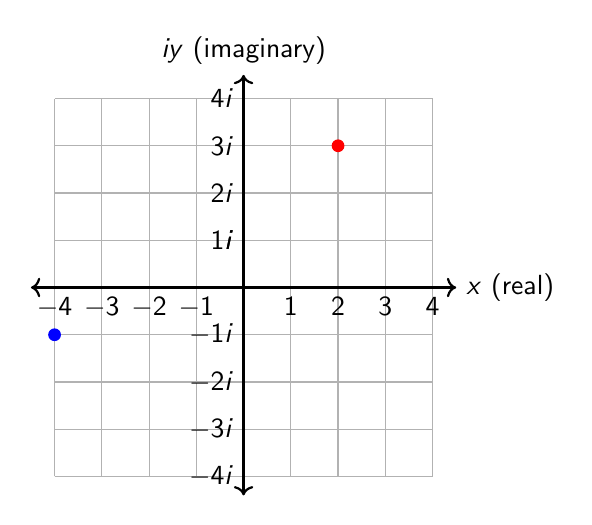
\begin{tikzpicture}[scale=0.6]
\draw [gray!60] (-4,-4) grid (4,4);
\draw [<->, thick] (-4.5,0) -- (4.5,0) node [right] {$x$ (real)};
\draw [<->, thick] (0,-4.4) -- (0,4.5) node [above] {$iy$ (imaginary)};
\foreach \x in {-4,-3,-2,-1,,1,2,3,4}
\node at (\x,0) [below] {$\small \x$};
\foreach \y in {-4,-3,-2,-1,,1,2,3,4}
\node at (0,\y) [left] {$\small \y i$};
\draw [color=red, fill=red] (2,3) circle [radius = 3.5pt];
\draw [color=blue, fill=blue] (-4,-1) circle [radius = 3.5pt];
\end{tikzpicture}
\end{center}

\vfill 
We can draw arrows (\textit{vectors}) from the origin to each point.

\begin{center}
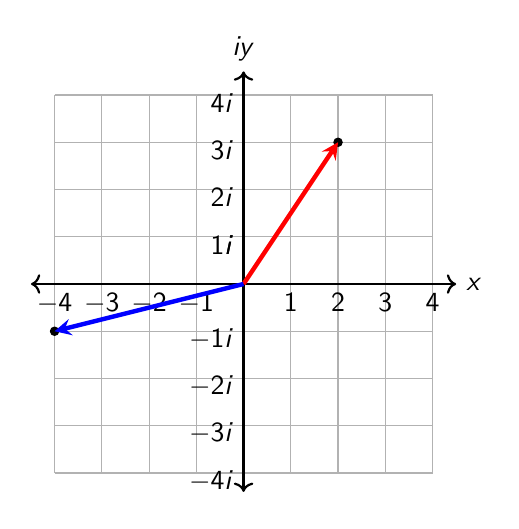
\begin{tikzpicture}[scale=0.6]
\draw [gray!60] (-4,-4) grid (4,4);
\draw [<->, thick] (-4.5,0) -- (4.5,0) node [right] {$x$};
\draw [<->, thick] (0,-4.4) -- (0,4.5) node [above] {$iy$};
\foreach \x in {-4,-3,-2,-1,,1,2,3,4}
\node at (\x,0) [below] {$\small \x$};
\foreach \y in {-4,-3,-2,-1,,1,2,3,4}
\node at (0,\y) [left, yshift=-0.1cm] {$\small \y i$};
\draw [fill=black] (2,3) circle [radius = 2.5pt];
\draw [fill=black] (-4,-1) circle [radius = 2.5pt];
\draw [->, red, ultra thick, >=stealth] (0,0) -- (2,3);
\draw [->, blue, ultra thick, >=stealth] (0,0) -- (-4,-1);
\end{tikzpicture}
\end{center}

\subsection*{Adding and Subtracting Complex Numbers}

\begin{itemize}
    \item Second arrow can start where first ends.
    \item Second arrow still points the same direction.
    \item You are just combining like terms.
\end{itemize}
\bigskip 

\begin{tabular}{p{0.5\textwidth}|p{0.4\textwidth}}
\parbox{3in}{For instance, ${\color{red}\pmb{(2 + 3i)}} + {\color{blue}\pmb{(-4 - i)}} = {\color{violet}\pmb{2 + 2i}}$ is shown below.}
&
For subtraction,
\begin{enumerate}
    \item Distribute the negative 
    \item Combine like terms
    \item ${\color{red}\pmb{(2 + 3i)}} - {\color{blue}\pmb{(-4 - i)}}$
\end{enumerate}
\\
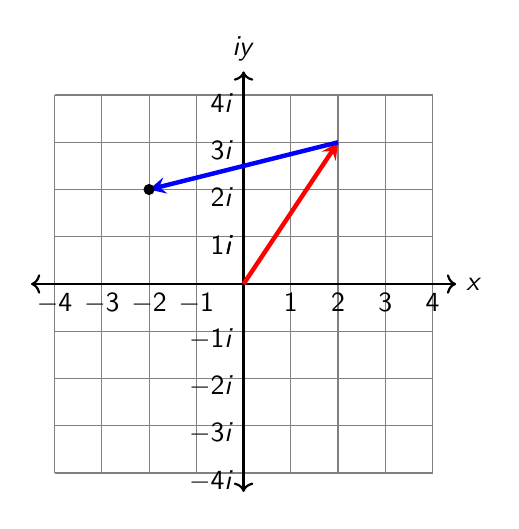
\begin{tikzpicture}[scale=0.6]
\draw [gray] (-4,-4) grid (4,4);
\draw [<->, thick] (-4.5,0) -- (4.5,0) node [right] {$x$};
\draw [<->, thick] (0,-4.4) -- (0,4.5) node [above] {$iy$};
\foreach \x in {-4,-3,-2,-1,,1,2,3,4}
\node at (\x,0) [below] {$\small \x$};
\foreach \y in {-4,-3,-2,-1,,1,2,3,4}
\node at (0,\y) [left, yshift=-0.1cm] {$\small \y i$};
\draw [->, red, ultra thick, >=stealth] (0,0) -- (2,3);
\draw [->, blue, ultra thick, >=stealth] (2,3) -- (-2,2);
\draw [fill=black] (-2,2) circle [radius = 3pt];
\end{tikzpicture}
&
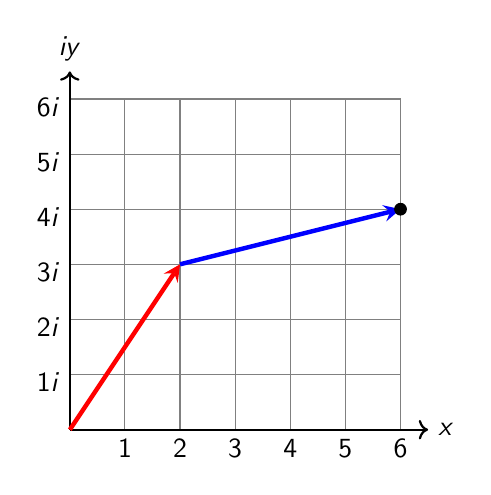
\begin{tikzpicture}[scale=0.7]
\draw [gray] (0,0) grid (6,6);
\draw [->, thick] (0,0) -- (6.5,0) node [right] {$x$};
\draw [->, thick] (0,0) -- (0,6.5) node [above] {$iy$};
\foreach \x in {1,2,...,6}
\node at (\x,0) [below] {$\small \x$};
\foreach \y in {1,2,...,6}
\node at (0,\y) [left, yshift=-0.1cm] {$\small \y i$};
\draw [->, red, ultra thick, >=stealth] (0,0) -- (2,3);
\draw [->, blue, ultra thick, >=stealth] (2,3) -- (6,4);
\draw [fill=black] (6,4) circle [radius = 3pt];
\end{tikzpicture}
\end{tabular}
\bigskip 

\begin{example}
Simplify each.
\begin{multicols}{2}
\begin{enumerate}[(a)]
    \item $(1 - 2i) + (3 + 4i)$
    \item $(1 - 2i) - (3 + 4i)$
\end{enumerate}
\end{multicols}
\end{example}

\newpage 

\subsection*{Multiplying Complex Numbers}

\begin{itemize}
    \item Multiply like normal
    \item Substitute $-1$ whenever you see an $i^2$
    \item Simplify and combine like terms
\end{itemize}

\begin{example}
Multiply and simplify each.
\begin{multicols}{2}
\begin{enumerate}[(a)]
    \item $(4 + 3i)(2 + i)$
    \item $(1 - 2i)(3 + 4i)$
\end{enumerate}
\end{multicols}
\end{example}


% Visually, let's see what happens when we multiply complex numbers $(4 + 3i)(2 + i)$:    \newline\\

% First, for $4 + 3i$, measure the length of the vector (in cm) and the angle it makes with the positive $x$-axis:

% \begin{center}
% \begin{tikzpicture}
% \draw [gray] (0,0) grid (6,6);
% \draw [->, thick] (0,0) -- (6.5,0) node [right] {$x$};
% \draw [->, thick] (0,0) -- (0,6.5) node [above] {$iy$};
% \foreach \x in {1,2,...,6}
% \node at (\x,0) [below] {$\small \x$};
% \foreach \y in {1,2,...,6}
% \node at (0,\y) [left, yshift=-0.1cm] {$\small \y i$};
% \draw [-Stealth, red, ultra thick] (0,0) -- (4,3);
% \draw [fill=black] (4,3) circle [radius = 3pt];
% \end{tikzpicture}
% \end{center}

% Now, let's do the same with the vector $2 + i$:

% \begin{center}
% \begin{tikzpicture}
% \draw [gray] (0,0) grid (6,6);
% \draw [->, thick] (0,0) -- (6.5,0) node [right] {$x$};
% \draw [->, thick] (0,0) -- (0,6.5) node [above] {$iy$};
% \foreach \x in {1,2,...,6}
% \node at (\x,0) [below] {$\small \x$};
% \foreach \y in {1,2,...,6}
% \node at (0,\y) [left, yshift=-0.1cm] {$\small \y i$};
% \draw [-Stealth, blue, ultra thick] (0,0) -- (2,1);
% \draw [fill=black] (2,1) circle [radius = 3pt];
% \end{tikzpicture}
% \end{center}

% \newpage

% Finally, measure the length (in cm) and angle of rotation with the positive $x$-axis for the answer to $(4 + 3i)(2 + i)$: $5 + 10i$

% \begin{center}
% \begin{tikzpicture}
% \draw [gray] (0,0) grid (6,10);
% \draw [->, thick] (0,0) -- (6.5,0) node [right] {$x$};
% \draw [->, thick] (0,0) -- (0,10.5) node [above] {$iy$};
% \foreach \x in {1,2,...,6}
% \node at (\x,0) [below] {$\small \x$};
% \foreach \y in {1,2,...,10}
% \node at (0,\y) [left, yshift=-0.1cm] {$\small \y i$};
% \draw [-Stealth, blue, ultra thick] (0,0) -- (5,10);
% \draw [fill=black] (5,10) circle [radius = 3pt];
% \end{tikzpicture}
% \end{center}

\vspace{3in}

\subsubsection*{Visual Intepretation of Multiplying Complex Numbers}

\begin{example}
\begin{enumerate}[(a)]
    \item Can you find a relationship between the lengths of $4 + 3i$ and $2 + i$ compared to the length of product?    \vspace{1in}
    \item Can you find a relationship between the angles that $4 + 3i$ and $2 + i$ make with the positive $x$-axis compared to the angle that the product makes?
\end{enumerate}
\end{example}
\newpage 

\subsection*{Dividing Complex Numbers}

Visually, what do you think happens with division? 
\vspace{0.25in} 

\begin{example}
Find the quotient of $\frac{4+3i}{2+i}$. 
\end{example}

\vspace{0.5in}

% \begin{center}
% \begin{tikzpicture}
% \draw [gray] (0,0) grid (6,6);
% \draw [->, thick] (0,0) -- (6.5,0) node [right] {$x$};
% \draw [->, thick] (0,0) -- (0,6.5) node [above] {$iy$};
% \foreach \x in {1,2,...,6}
% \node at (\x,0) [below] {$\small \x$};
% \foreach \y in {1,2,...,6}
% \node at (0,\y) [left, yshift=-0.1cm] {$\small \y i$};
% \end{tikzpicture}
% \end{center}

% Now, suppose we don't want to draw out every single division problem. How can we get an answer that is more-accurate than our graph? \vspace{1in}

% Also, if we substitute $i = \sqrt{-1}$, for the above, we will still get square roots in the denominator (a big no-no in math):
% \[
% \frac{4+3\sqrt{-1}}{2+\sqrt{-1}}
% \]

\begin{tcolorbox}[colframe=green!70!white, coltitle=black, title=\textbf{Complex Conjugate}]
The \textbf{complex conjugate} of a complex number in the form 
\[ z = a + bi \]
is $\overline{z} = a - bi$ and vice versa.
\end{tcolorbox}
\bigskip 

% The below illustrates the complex conjugate of $2 + i$, which is $2 - i$:

% \begin{center}
% \begin{tikzpicture}
% \draw [gray] (0,-3) grid (5,3);
% \draw [->, thick] (0,0) -- (5.5,0) node [right] {$x$};
% \draw [->, thick] (0,-3) -- (0,3.5) node [above] {$iy$};
% \foreach \x in {1,2,3,4,5}
% \node at (\x,0) [below] {$\small \x$};
% \foreach \y in {-3,-2,-1,,1,2,3}
% \node at (0,\y) [left, yshift=-0.1cm] {$\small \y i$};
% \draw [fill=black] (2,1) circle [radius=2pt];
% \draw [fill=black] (2,-1) circle [radius=2pt];
% \draw [-stealth, red, very thick] (0,0) -- (2,1);
% \draw [-stealth, blue, very thick] (0,0) -- (2,-1);
% \end{tikzpicture}
% \end{center}

\begin{example}
Find and graph the product of $(2 + i)(2 - i)$. \newline

\begin{tikzpicture}
\draw [dotted] (-2,-2) grid (6,2);
\draw [->, thick] (-2.5,0) -- (6.5,0) node [right] {$x$};
\draw [->, thick] (0,-2.5) -- (0,2.5) node [above] {$iy$};
\foreach \x in {-2,-1,1,2,3,4,5,6}
\node at (\x,0) [below] {$\x$};
\foreach \y in {-2,-1,1,2}
\node at (0,\y) [left, yshift=-0.1cm] {$\y i$};
\end{tikzpicture}
\end{example}
\bigskip  

To divide complex numbers, you multiply the numerator and denominator by the \emph{conjugate} of the denominator.
\bigskip 

\begin{example}
Divide each.
\begin{multicols}{2}
\begin{enumerate}[(a)]
    \item $\dfrac{4+3i}{2+i}$
    \item $\dfrac{1-2i}{3+4i}$
\end{enumerate}
\end{multicols}
\end{example}

\vfill 
\newpage 

\parbox{4in}{We can even use complex numbers to solve quadratic equations 
when the graph of the equation does not intersect the $x$-axis.}
\bigskip 

\begin{example}
Solve each. None of these problems are factorable.
\begin{enumerate}[(a)]
\begin{multicols}{2}
    \item $x^2 + 4x + 8 = 0$
    \item $12x^2-12x+12 = 0$
\end{multicols}
\vfill 
\begin{multicols}{2}
    \item $9x^2 + 5x + 14 = 3$
    \item $-4x^2 - 4x + 18 = -10x^2 + 7x + 6$
\end{multicols}
\end{enumerate}
\end{example}
\vfill 

\end{document}
